\section{Benchmarks}
\label{sec:bench}

We now compare the performances of our implementations according to two criterions.
First, we compare the successive algorithmic refinements using the \haskell
implementation presented in \cref{sec:motivation} and \cref{sec:improvements}.
We then compare different data-structure implementations for segments
using the \ocaml implementation detailed in \cref{sec:ocaml}.

All benchmarks were done on a ThinkPad T470 with an i5-7200U CPU and 12Go of memory.
The \haskell benchmarks use the lts-10.8 platform and the \texttt{-02} option.
The OCaml benchmarks use \ocaml 4.06.1 with the flambda optimizer and the
\texttt{-03} option. Additionally, we annotated functors
with the \code{[@inline]} annotation which ensures that functors are applied at
compile-time and their content benefits from available optimizations.

\subsection{Comparing algorithms in the \haskell implementation}

\cref{sec:motivation} and \cref{sec:improvements} present improvements to
the algorithm for generating languages. We now evaluate
the impact of these improvements on performances.
The performances are obviously highly dependent on the regular expression
considered. We chose three regular expressions that highlight
the various strength and weaknesses of the different approaches:
\begin{itemize}
\item$\Rstar a$: The \code{star} operation is very performance intensive.
  The input language only contains one segment, which highlight the usefulness
  of sparse indexing and maps. Since each segments of the output language contains
  only one element, this also tests the behavior of star at high length.
\item $\Rstar{(\Rconcat{a}{\Rstar{b}})}$: On the opposite end of the spectrum, this
  regular expression applies \code{star} to a language where all segments
  are neither empty nor full. This measures the performances of \code{star}
  and \code{concatenation} on non-sparse languages.
\item $\Rconcat{\Rcomplement{(\Rstar{a})}}{b}$: Finally, this regular expressions
  tests the generation of a very big language through \code{star} and the
  concatenation to a much smaller language.
\end{itemize}

\TODO{Describe what are the different haskell implementations: naive, ref, seg, refConv, segConv}

To evaluate the performance, we iterate through the stream of words produced by
the generator. Every 20 words, we register the time since the start of the
iteration. We stop the iteration after 5 seconds and graph the numbers reached in
function of the time spent: the faster a curve grows, the faster it generate
words.
The results can be seen in \cref{bench:haskell:all}.
We first note that most implementations generate between 3000 and
150000 words in the first second, which seems more than sufficient for testing
purposes.
Additionally, the refConv implementation
which uses symbolic segments and convolutions
is the most versatile. This validates our improvements
proposed in \cref{sec:improvements}.
Looking at each graph in more details, we can make the following remarks:
\begin{itemize}[leftmargin=*]
\item All implementations are equally fast on $\Rstar a$ except
for the naive implementation. This is not surprising, since it does not uses
sparse indexing and only relies on list lookups.
\item 
For $\Rstar{(\Rconcat{a}{\Rstar{b}})}$ and
$\Rconcat{\Rcomplement{(\Rstar{a})}}{b}$, some implementations showcase
a shape in ``skewed stairs''. This is explained by insufficient laziness:
when arriving at a new segment, part of the work is done eagerly which causes
a plateau. When that part is done, the enumeration proceeds lazily.
Since laziness and GHC optimizations are hard to control in a manual fashion,
we did not attempt to correct this.
\item $\Rstar{(\Rconcat{a}{\Rstar{b}})}$ demonstrates that sparse indexing
  does degrade performances when applying \code{star} to non-sparse languages.
  The performance impact is however recovered using the convolution technique
  presented in \cref{sec:convolution}.
\item The ref and refConv algorithm are significantly faster
  on $\Rconcat{\Rcomplement{(\Rstar{a})}}{b}$ compared to the
  seg and SegConv. This is probably explained by
  the symbolic treatment of segments. Complement is implemented
  as the difference with $\Rstar{\Sigma}$ which can be represented much more
  compactly in a symbolic manner.
\end{itemize}

\begin{figure}[h]
  \centering
  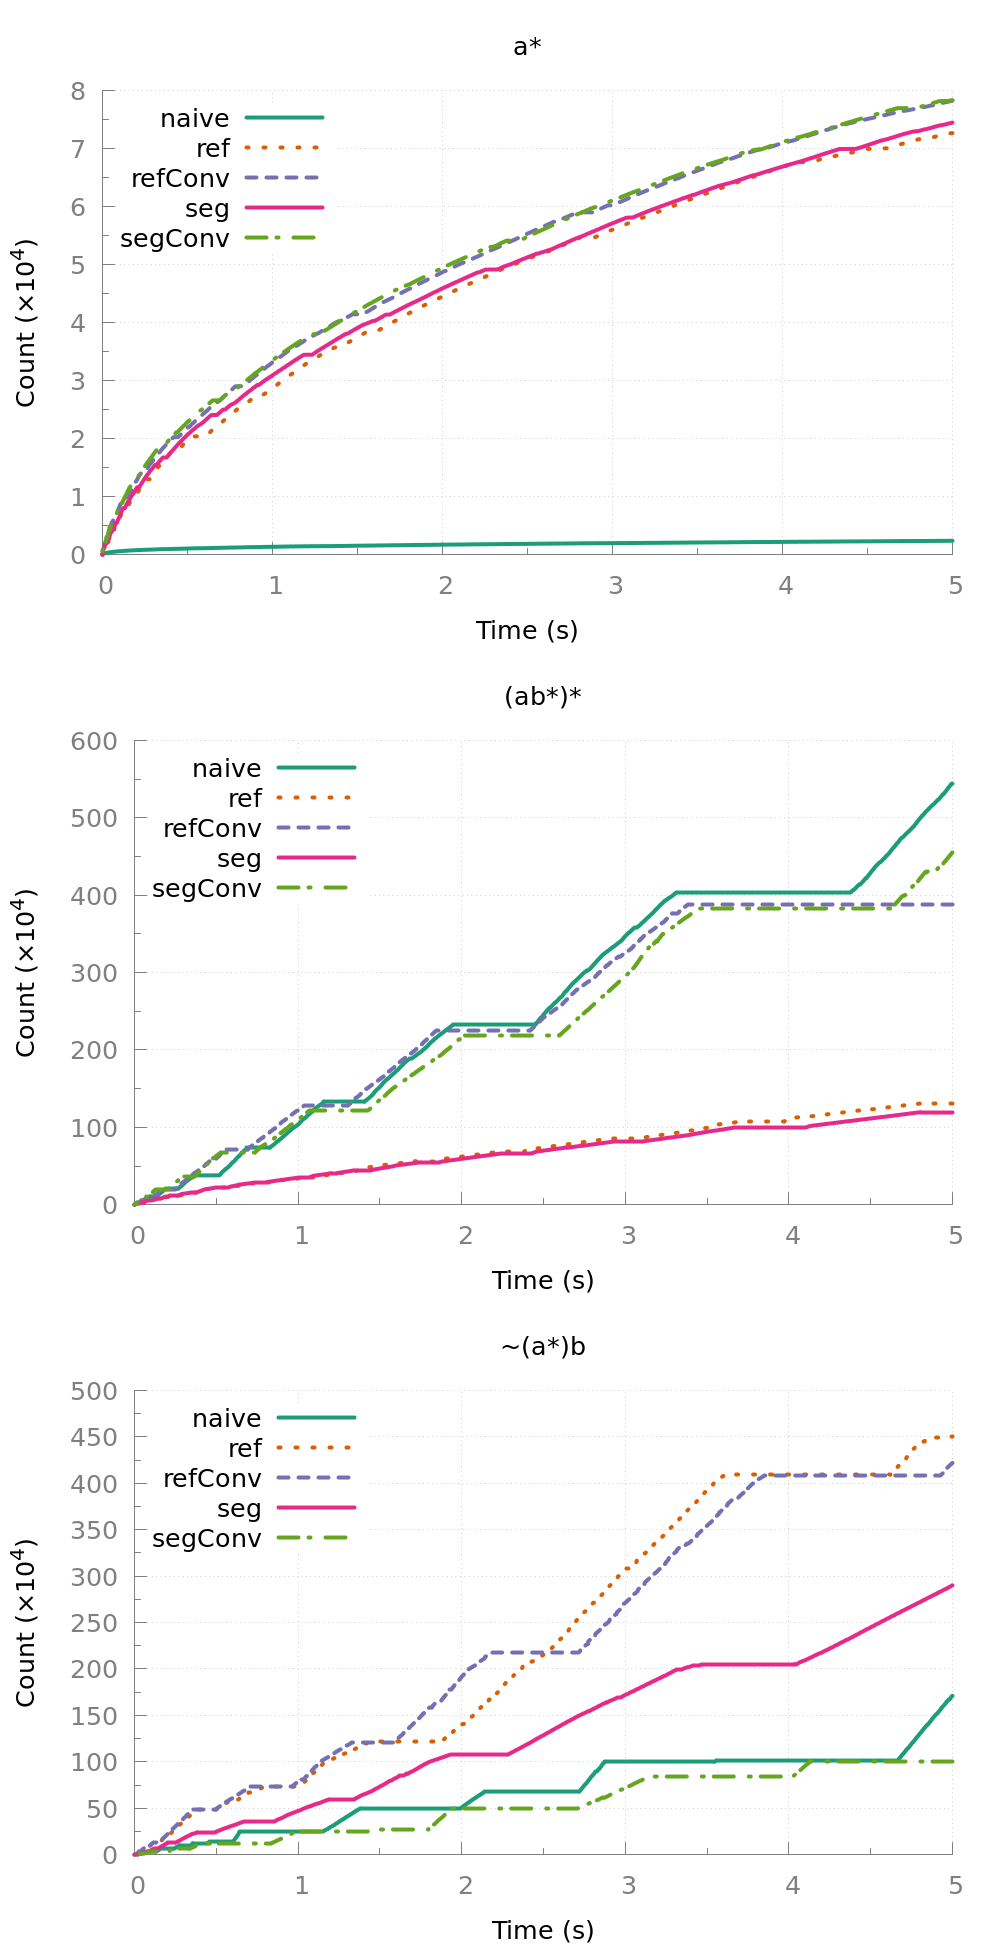
\includegraphics[height=0.33\linewidth]{measure/haskell_all.png}
  \caption{Benchmark for the \haskell implementation with various algorithms}
  \label{bench:haskell:all}
\end{figure}

\subsection{Comparing data-structures in the \ocaml implementation}
\label{sec:bench:ocaml}

We have now established that the refConv algorithm provides the best performances.
The \haskell implementation, however, only uses lazy lists. To measure
the influence of strictness and data-structure on language generation,
we turn to the functorized \ocaml implementation.
We follow the same methodology than the \haskell evaluation using
the regular expressions
$\Rstar a$, $\Rstar{(\Rconcat{a}{\Rstar{b}})}$ and
$\Rconcat{\Rcomplement{(\Rstar{a})}}{b}$.
The results are shown in \cref{bench:ocaml:all}.

\begin{figure}[b]
  \centering
  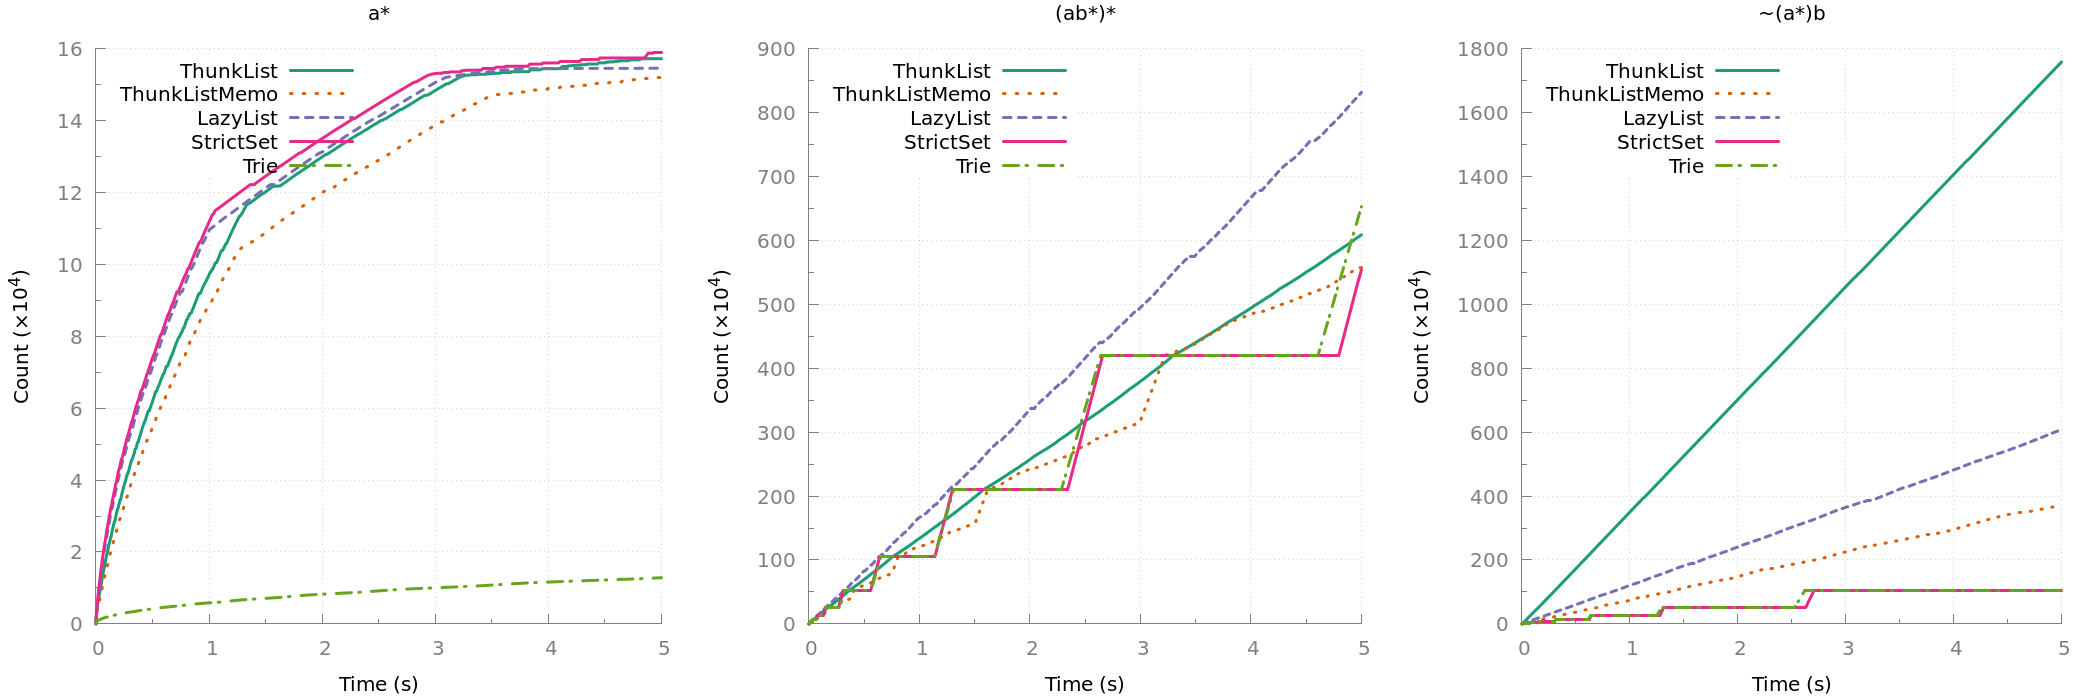
\includegraphics[height=0.33\linewidth]{measure/ocaml_all.png}
  \caption{Benchmark for the \ocaml implementation with various data-structures}
  \label{bench:ocaml:all}
  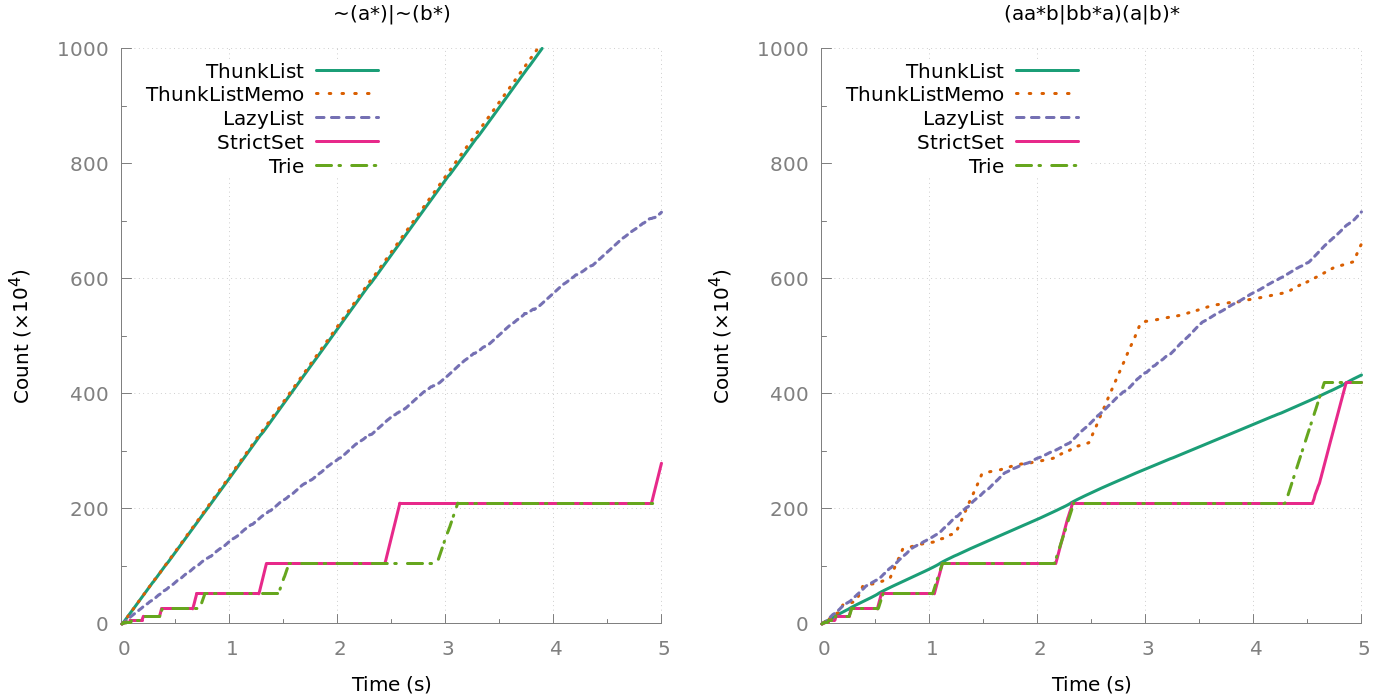
\includegraphics[height=0.33\linewidth]{measure/ocaml_union.png}
  \caption{Benchmarking \texttt{union} in the \ocaml data-structures}
  \label{bench:ocaml:union}
\end{figure}

Unlike the previous benchmark for algorithms, there is no clearly winner
among data-structures. The \code{ThunkList} and \code{LazyList} modules seem to
be superior to the alternatives, although the result are highly influenced by
the regular expression considered:
\begin{itemize}[leftmargin=*]
\item The \code{Trie} module is very inefficient on $\Rstar a$. Unfortunately,
  our implementation of tries doesn't use path compression. Each
  branch is only labeled by a single character.
  In the case of $\Rstar a$, each segment contains only one word and the
  trie degenerates to a list of character.
  We believe
  an implementation of tries with path compressions would perform similarly to
  the other data-structures.
\item The other data-structures on $\Rstar a$ exhibit a very pronounced slowdown
  when reaching 150000 words.
  We believe this is due to garbage collection: indeed
  all data-structure were consuming up to 10Go of memory before
  a collection was triggered. Memory consumption for the other regular
  expressions was far less significant.
\item Strict data-structure showcase a very marked ``skewed stair'' pattern.
  This pattern is however completely absent for \code{ThunkList} and
  \code{LazyList}. This demonstrates, if that was still needed,
  that laziness does indeed work very well in \ocaml. These results also confirm
  that strict data-structures should only be used when one wants to obtain
  all the elements up to a given length, in which case the stair pattern
  doesn't cause any penalty.
\item Memoization for thunk lists significantly decreases performances. It seems
  that the linear cost of memoizing the thunk list and allocating the vectors
  is higher than simple recomputing lists.
\end{itemize}

While the regular expressions presented previously do exercise
\code{concatenation} and \code{star}, they do not exercise set operations.
In order to test set operations on non-trivial segments (segments that
are neither full nor empty), we consider the language of words with at least
one $a$ and one $b$. This language can be built in two ways:
$\Runion{\Rcomplement{\Rstar{a}}}{\Rcomplement{\Rstar{b}}}$ and
$\Rconcat{(\Runion{a\Rstar{a}b}{b\Rstar{b}a})}{\Rstar{\Sigma}}$.
The first applies \code{union} to two large languages, the second takes
the union of smaller languages, but uses a concatenation.
The performances of the various data-structure on these two regular expressions
are presented in \cref{bench:ocaml:union}.
Lazy and thunk lists, with memoization or not, are very efficient on the union of languages but less so when concatenation is involved. Performance of strict sets and tries is surprisingly poor.

\subsection{The influence of regular expressions on performances}

As we have seen on the various benchmarks, the performance of the language
generator highly depends on the precise structure of both
the generated language and the regular expression considered.
We attempt to explore this remark by comparing various regular expressions
with the \code{refConv} \haskell implementation and the \code{ThunkList}
\ocaml implementation.
Before presenting the results, a word of warning:
We do not claim to offer a fair comparison between languages!
The two implementations are not exactly the same and we made no attempt
to measure both language in exactly the same conditions.
The comparison is shown in \cref{bench:langs}. In order to better visualize the
various regular expressions, the word count uses a logarithmic scale.

In addition to the regular expressions presented previously, we added the following:
\begin{itemize}
\item $\Rstar{(\Sigma\Sigma)}$, the language of words of lenght pair. This language
  is neither finite nor cofinite and make great use of the symbolic
  representation of segments.
\item $\Rstar{(\Runion{1 \Rstar{(0\Rstar{1}0)}1}{0})}$, the language
  of multiple of 3 written in binary. Again, this is a language that is neither
  finite nor cofinite, but its segments are never full nor empty.
\item $\Rstar{a}b$ and $b\Rstar{a}$, which allow us to see if
  \code{concatenation} has symmetric performances.
\end{itemize}

We remark that languages are roughly ordered by size. It is faster
to generate a language whose segments are bigger. Indeed,
most of the operations, notably
those involving product of segments, are more expansive when considering
segments of higher indices, thus making longer strings harder to generate.
If each segment contain many words, we do not need to compute many segments to
generate a large number of words.
%
We also note that the generation of $\Rstar{a}b$ and $b\Rstar{a}$
has indeed the same performance in the \haskell implementation.
The \ocaml version is however asymmetric, since it does not implement
the improved convolution technique with
detection of finite languages, as described in \cref{sec:convolution}.


\begin{figure}[h]
  \centering
  \begin{subfigure}[t]{0.45\linewidth}
    \centering
    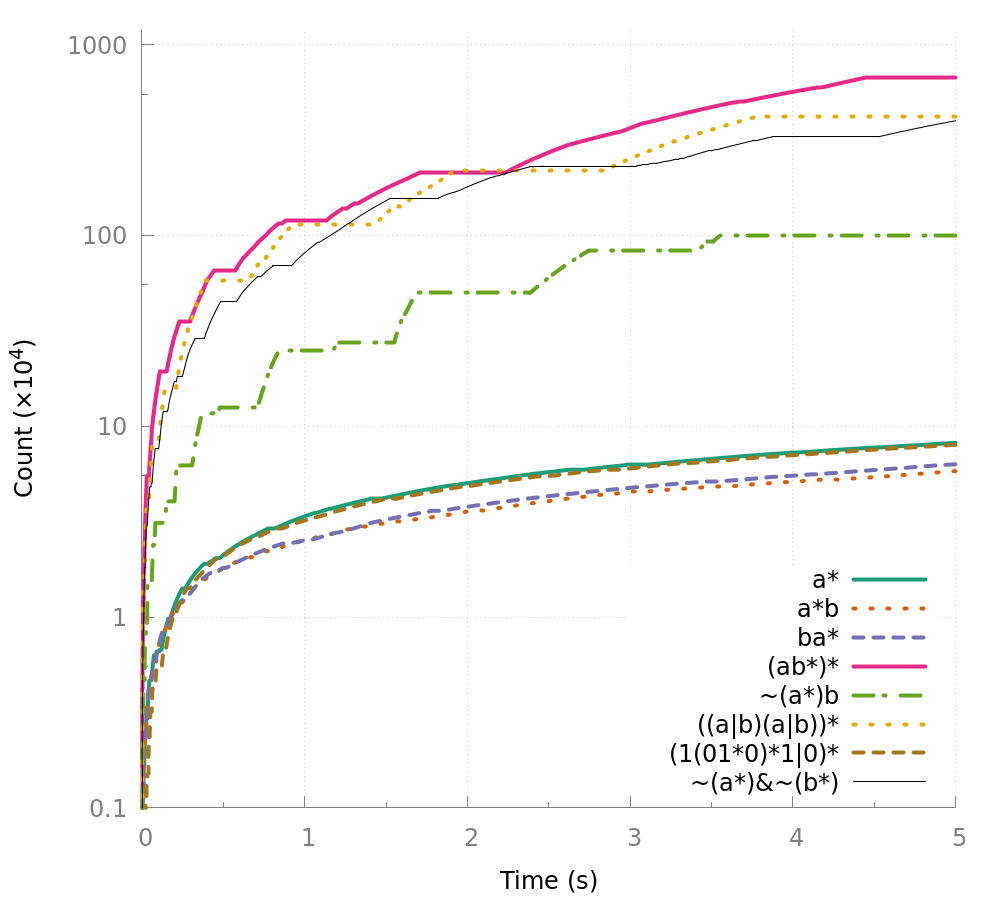
\includegraphics[width=\linewidth]{measure/haskell_langs.png}
    \caption{\haskell implementation with \code{segConv}}
    \label{bench:haskell:langs}
  \end{subfigure}
  \begin{subfigure}[t]{0.45\linewidth}
    \centering
    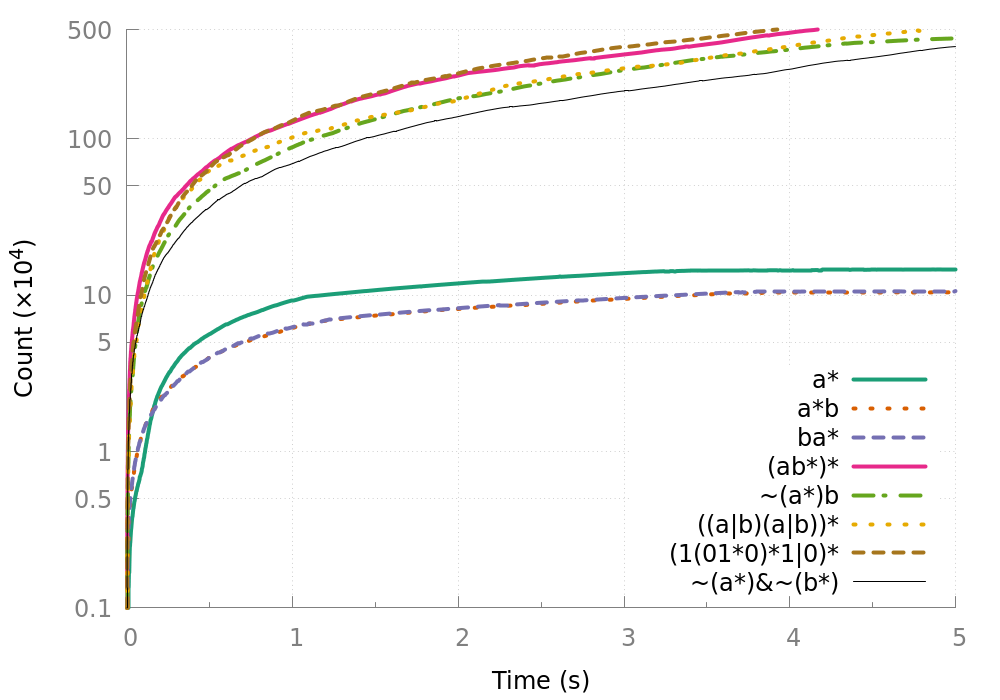
\includegraphics[width=\linewidth]{measure/ocaml_langs.png}
    \caption{\ocaml implementation with \code{ThunkList}}
    \label{bench:ocaml:langs}
  \end{subfigure}
  \caption{Benchmark on different regular expressions}
  \label{bench:langs}
\end{figure}

%%% Local Variables:
%%% mode: latex
%%% TeX-master: "main"
%%% End:
